\documentclass[iop]{emulateapj}

\newcommand{\vdag}{(v)^\dahher}
\newcommand{\myemail}{skywalker@galaxy.far.far.away}


\shorttitle{Detecting Assembly Bias in Massive Galaxy Clusters}
\shortauthors{E. Molina}

\usepackage{graphicx}
\usepackage{gensymb}
\usepackage{float}

\begin{document}

\title{Non-Detection of Assembly Bias as a function of Brightest Cluster Galaxy Ellipticity}


\author{Eden Molina}
\affil{University of California, Los Angeles \\
Jet Propulsion Laboratory \\ California Institute of Technology, Pasadena, CA 91109, USA}
\author{Jason Rhodes}
\affil{Jet Propulsion Laboratory \\ California Institute of Technology, Pasadena, CA 91109, USA}
\and

\author{Hironao Miyatake}
\affil{Jet Propulsion Laboratory \\ California Institute of Technology, Pasadena, CA 91109, USA}

\begin{abstract}
\noindent Galaxies and galaxy clusters are formed in dark matter halos. The clustering of the dark matter halos is enhanced against that of underlying dark matter distribution, this phenomena is known as bias. It has been observed that halo bias depends on halo mass.  However, theoretical and numerical studies have shown that bias can depend on halo properties other than mass. This is known as assembly bias. In this project 8,648 Sloan Digital Sky Survey (SDSS) red-sequence DR8 Matched-filter Probabilistic Percolaion (redMaPPer) galaxy clusters were divided into two subsamples based on the  brightest cluster galaxy (BCG)  ellipticity---large and small. Weak lensing was used to verify that the mass of the subsamples are the same because it directly probes the mass of the matter including dark matter. This objective of this project is to detect if assembly bias correlates to BCG ellipticity on the assumption that dark matter ellipticity correlates to BCG ellipticity. After the weak lensing and the clustering signal were calculated it was found that there was no evidence of assembly bias correlated with BCG ellipticity.
\end{abstract}

%\keywords{globular clusters: general ---
%globular clusters: individual(\objectname{NGC 6397},
%\object{NGC 6624}, \objectname[M 15]{NGC 7078},
%\object[Cl 1938-341]{Terzan 8})}

\section{Introduction}
Dark energy and dark matter contribute about 95\% of the matter and energy in the universe. Dark matter allows for the formation of large scale structures such as galaxies and galaxy clusters. Dark energy is responsible for the accelerating expansion of the universe.

Cosmological information about the nature of dark matter and dark energy can be extracted by using a two point matter auto-correlation function. The matter auto-correlation function is defined in terms of the matter density fluctuation $\delta_m = \frac{\rho_m} {\overline{\rho}_m} - 1$ as
	\begin{equation}
		\label{eq:dark_matter_correlation}
		\xi_{mm}(r) = \langle  \delta_m (x) \delta_m^* (x+r) \rangle,
	\end{equation}
where $\rho_m$ is the matter density at a given position, while $\overline{\rho_m}$ is the average matter fluctuation of the universe.
Unfortunately we cannot directly measure $\xi_{mm}$, the clustering of the dark matter. However, the cosmological information is imprinted in the galaxy cluster distribution, since clusters are formed in dark matter halos. Dark matter halos are formed when the matter density fluctuation $\delta$ exceeds a certain threshold. To extract the cosmological information from the distribution of clusters, we need to relate the cluster distribution with dark matter distribution. At large scales, fluctuations of dark matter density and cluster number density can be related by using linear bias parameter $b$:
	\begin{equation}
		\label{eq:Assumption}
		\delta_h = b \delta_m.
	\end{equation}

The cluster correlation can also be defined in terms of the correlation functions above. The correlation of the dark matter distribution should take the form of eq (\ref{eq:dark_matter_correlation}). Subsequently, the correlation of galaxy clusters can be calculated by taking the correlation of the number density fluctuation:
	\begin{equation}
		\label{eq:galaxy_light_correlation}
		\xi_{hh} = \langle \delta_h (x) \delta_{g}^*(x+r) \rangle.
	\end{equation}
In order to extract information about the dark matter distribution from the galaxy light, eqs (\ref{eq:dark_matter_correlation}) \& (\ref{eq:galaxy_light_correlation}) must be related so that observation and theory can be equated.

Using the bias parameter in eq (\ref{eq:Assumption}), eq (\ref{eq:galaxy_light_correlation}) can take the form:
	\begin{equation}
		\label{eq:fCorrelation}
		\xi_{hh} = b^2 \langle \delta_m (x) \delta_{m}^*(x+r) \rangle.
	\end{equation}
	
The bias primarily depends on halo mass, which is confirmed by observational studies. Theoretical and numerical studies have shown that bias can depend on properties other than mass such as BCG ellipticity and BCG color (\cite{2008ApJ...687...12D}; \cite{2014ApJ...785..104R}), which is called assembly bias. However, assembly bias has not been observed for a decade.

\cite{2016PhRvL.116d1301M} firstly reported the evidence of assembly bias. They divided a sample of Sloan Digital Sky Survey (SDSS) red-sequence DR8 Matched-filter Probabilistic Percolation (redMaPPer) galaxy clusters (\cite{2011ApJS..193...29A}; \cite{2014ApJ...785..104R}) of redshift 0.10  $<$ z $<$ 0.33 into two subsamples based on the average distance of each member galaxy from the brightest cluster galaxy (BCG), $\langle R_{mem} \rangle$. This value quantifies how separated the member galaxies are within a cluster. The median $\langle R_{mem} \rangle$ was calculated and each individual cluster was placed in a subsample whose  $\langle R_{mem} \rangle$ is higher or lower than the average. Once the subsamples were created, the weak lensing signal was calculated. The weak lensing will allow for measuring matter distribution (including dark matter) around clusters. The lensing signals at scales $<$ 10$h^{-1} \mathrm{Mpc}$ have similar amplitudes, which confirmed the subsamples had approximately the same mass, and a difference at 2.5--$\sigma$ significance on scales $>$ 10 $h^{-1} \mathrm{Mpc}$ suggested the presence of assembly bias. They also looked into clustering of clusters, which displayed a significant difference (4.4--$\sigma$ difference) and hence evidence of assembly bias.

The main goal of this project is to detect assembly bias in massive clusters through BCG ellipticity, following the measurement scheme in \cite{2016PhRvL.116d1301M}. This research was conducted at the Jet Propulsion Laboratory--California Institute of Technology, under a contract with the National Aeronautics and Space Administration.

\section{Data}
\subsection{Galaxy Cluster Catalog}
In this project 8,648 SDSS redMaPPer galaxy clusters in the redshift range of 0.10 $<$ z $<$ 0.33 and optical richness $\lambda$ of $>$20 were studied.

In order to correct for systematic errors in the lensing signal and to calculate the clustering signal, we used the random points which were generated in a way that their redshift and richness follow a similar distribution to an observed sample of cluster. The 100 random realizations were generated in order to reduce statistical uncertainties.


\subsection{Subsample Division}
The 8,648 galaxy clusters were divided into 2 subsamples based on the BCG ellipticity--the axis ratio. Since there are BCG ellipticity measured on three different bands (gri, \cite{1996AJ....111.1748F}), there are a total of 6 subsamples. Based on the median BCG ellipticity a cluster lied above or below that median. The two subsamples are respectively labeled large and small ellipticities in this paper. 
	\begin{figure*}[h]
		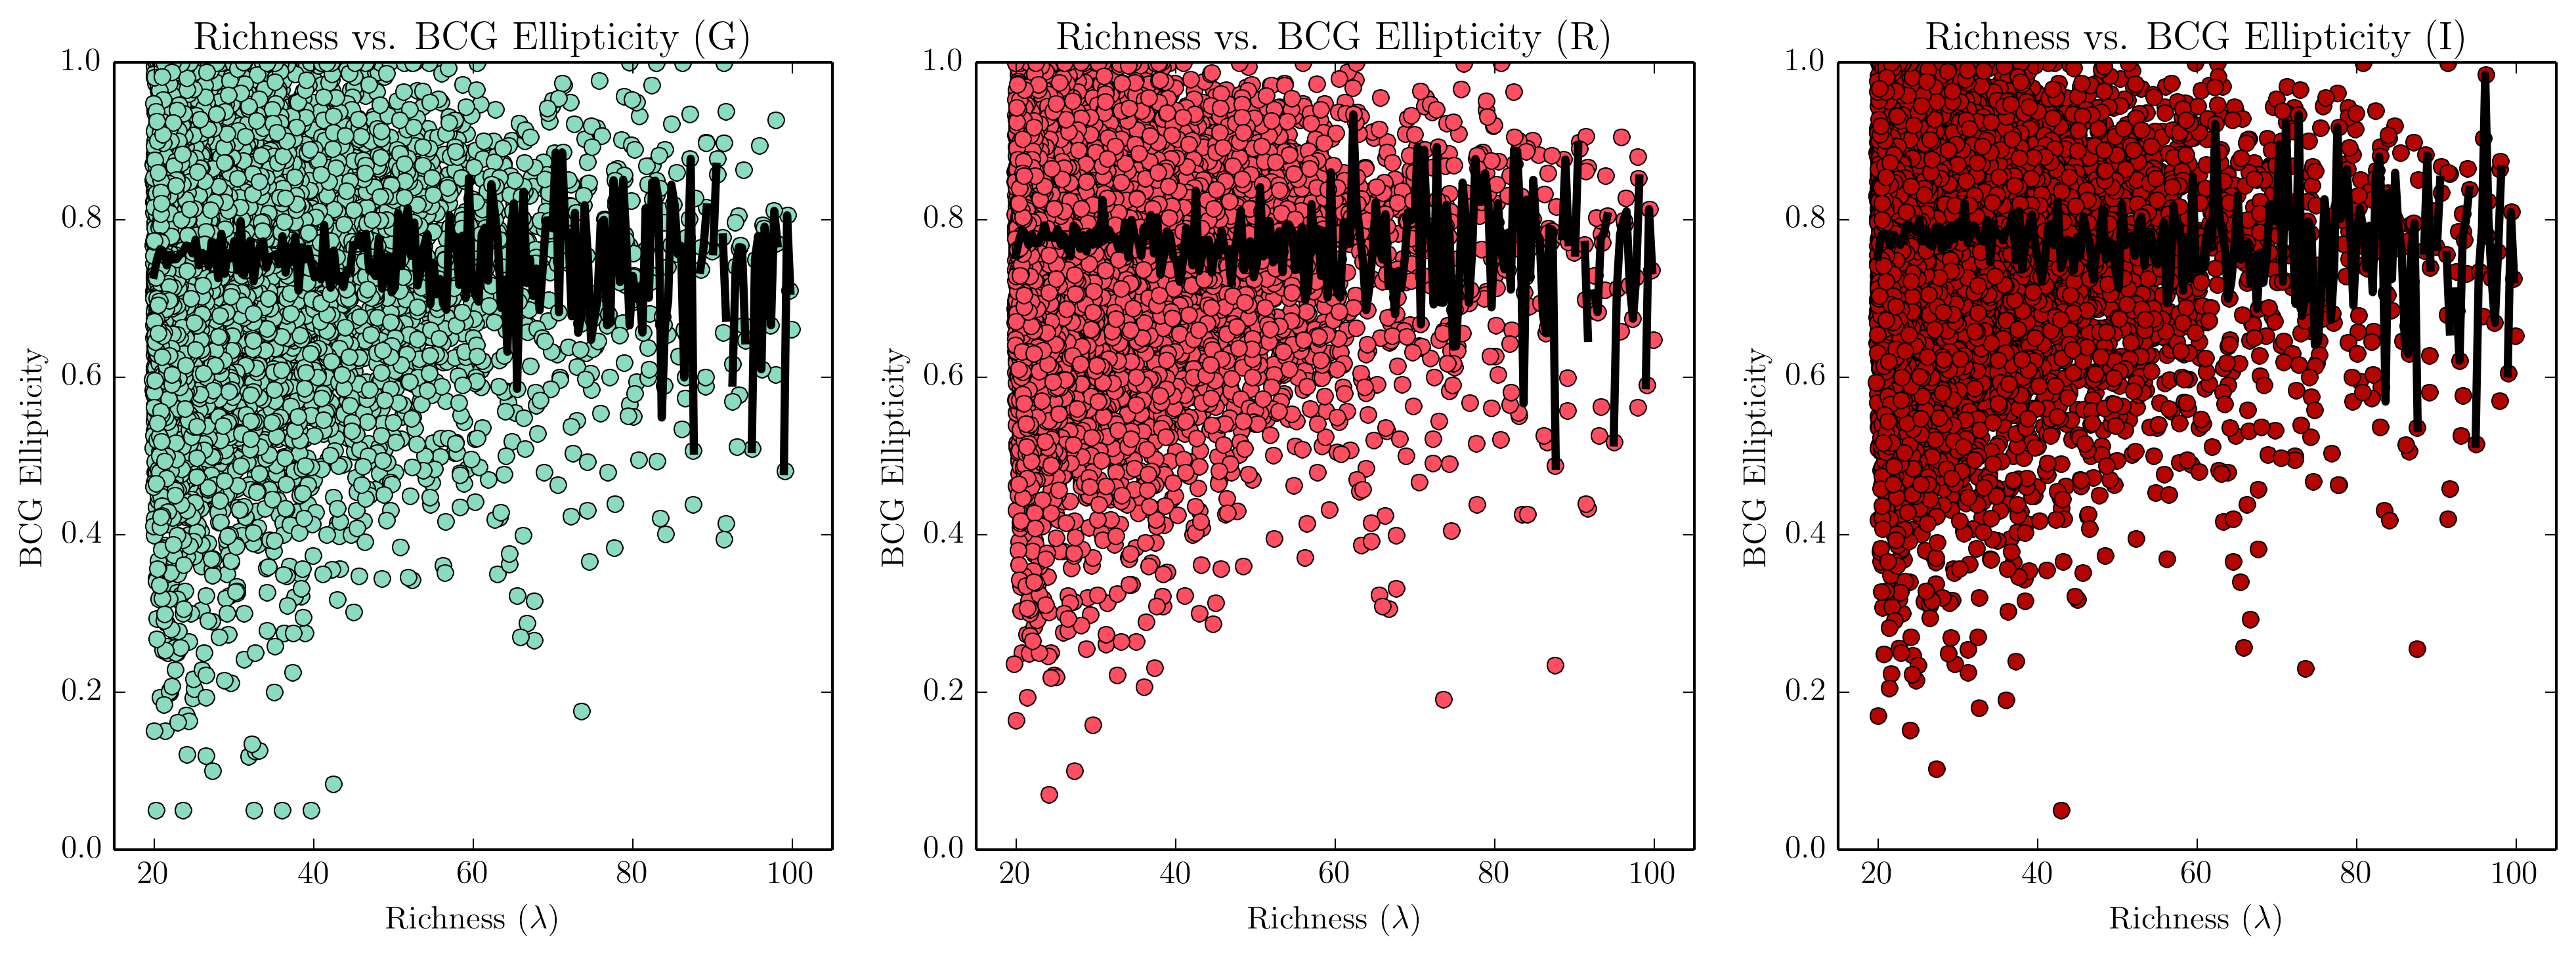
\includegraphics[width = \linewidth]{Richness}
		\label{fig:Richness}
		\caption{Scatter plot of BCG Ellipticity vs. Richness ($\lambda$) Richness is correlated with mass, a straight median line between the varying values of Richness indicates that BCG Ellipticity and Mass are not correlated. This check is vital to the project because BCG ellipticity cannot depend on mass.}
	\end{figure*}\label{fig:Redshift}
	
	\begin{figure*}[h]
		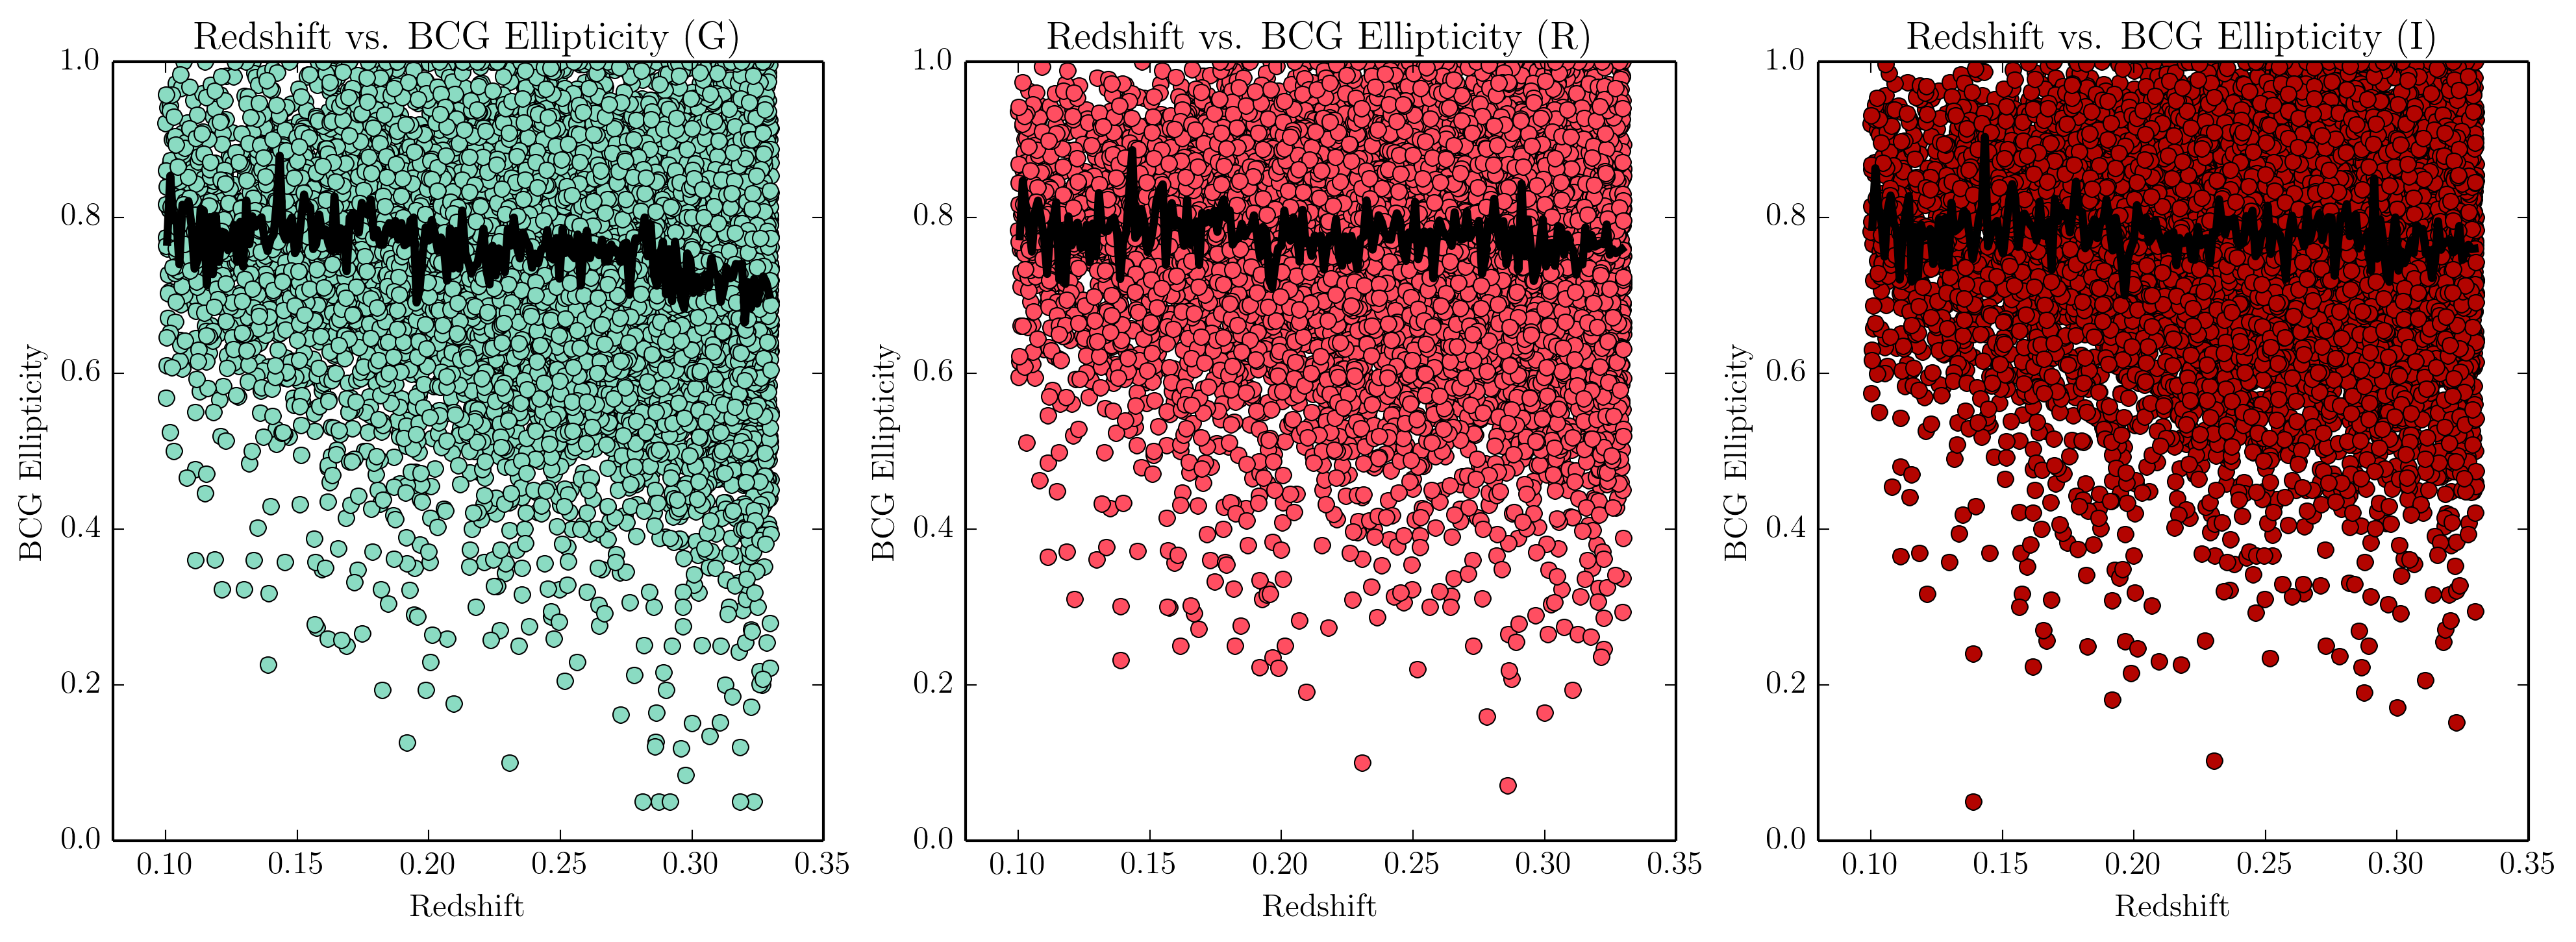
\includegraphics[width = \linewidth]{Redshift}
		\caption{Scatter plot of BCG Ellipticity vs. Redshift ($\lambda$). From the black median line, it can be inferred that there is no correlation between BCG ellipticity and Redshift.}
	\end{figure*}
In order to proceed the analysis for assembly bias, the two cluster subsamples must have the same mass. This is done in order to get rid of  the dependence on mass with which bias is known to be strongly correlated. Getting rid of mass dependance allows us to analyze the other properties of galaxy clusters. A preliminary check for mass independence can be done by plotting the median line on the scatter plot displaying BCG Ellipticity vs. Richness ($\lambda$) and Redshift (z) shown on Figures 1 and 2 respectively. %Display plot of the histogram here%

Because the median line of the scatter plots are fairly straight, we can infer that there is no correlation between the masses of the subgroups. However, we cannot definitively state the masses of the subsamples are the same until the weak lensing signal is plotted. This is because one of the plots relates ellipticity and richness($\lambda$). Richness, or optical richness, is the number of member galaxies in a cluster above a certain luminosity threshold. Using richness to determine the mass of a galaxy cluster only provides us a rough estimate of the cluster mass, since it does not directly measure dark matter distribution around a cluster.

Redshift was also checked to have no correlation with ellipticity because bias also depends on redshift. Figure 2 shows that there is no correlation between BCG ellipticity and redshift, therefore we can proceed with the study.

%Section 3: Measurement
\section{Measurement}
\subsection{Weak Lensing}

Weak lensing is used in this project to probe the dark matter distribution. According to general relativity mass bends space-time. The more mass at a particular region in space, the more space-time will be distorted. Consequently because light travels along space-time, its path will be bent along the curvature of a mass and its image will be distorted (or lensed) when all the light arrives at an observer.  The more lensed an image is, the more mass there will be between the object(galaxy/galaxy cluster) and the observer.
\subsubsection{Basics of Weak Lensing}

The weak lensing signal in this paper can be calculated by
	\begin{equation}\label{eq:DeltaSigma}
		\Delta \Sigma(R) = \Delta\Sigma_{crit}\times\gamma_{t}(R)
	\end{equation}
where $\Delta\Sigma_{crit}$ is the critical mass density that can be expressed in terms of redshift, and $\gamma_{t}(R)$ is the lensing distortion. (\cite{2015ApJ...806....1M})
	\begin{equation} \label{eq:DeltaSigmaR}
		\Delta\Sigma_{crit} = \frac{c^2} {4\pi G}\frac{D_{A} (z_{s})}{D_{A}(z_l , z_s) D_A (z_l) }.
	\end{equation}
In eq (\ref{eq:DeltaSigmaR}), $D_{A} (z_{s})$ represents the distance from the observer to a source galaxy behind a lensing cluster, $D_{A}(z_l , z_s)$ is the angular diameter distance from a lensing cluster to a source galaxy, and $D_A (z_l)$ is the angular distance from the observer to a lensing cluster.

The lensing signal is a statistical measurement that is estimated by stacking the tangental component of the source galaxy ellipticities with respect to the lens clusters. $\Delta\Sigma$(R) is calculated using lens-source pairs (ls):
	\begin{equation}
		\Delta \Sigma (R) = \frac{\Sigma_{ls}w_{ls} e_t ^{ls} \Sigma_{c,ls} } {2 \mathrm{R} \Sigma_{rs} w_{rs}},
		\label{eq:DeltaSigmaEllip}
	\end{equation}
where $e_t$ is the tangental component of ellipticity of source galaxies, and $w$ is the weight of a lens-source pair. The factor R comes from the summation rule of ellipticity.

\subsubsection{Contamination by Physically-associated Galaxies}
	Galaxies physically associated with lens clusters can be selected as source galaxies. The physically-associated galaxies will dilute the lensing signal because they are not lensed, but they are being counted as galaxies contributing to the lensing.  A correction factor for this contamination, which is called boost factor can be estimated by comparing the counts of source galaxies behind the lens to that behind the random points.
	\begin{equation}
		B(R) = \frac{\Sigma_{ls} w_l w_s (\langle \Sigma_{cr}^{-1} \rangle^{(ls)})^2 / \Sigma_l w_l} {\Sigma_{rs} w_r w_s(\langle \Sigma_{cr}^{-1} \rangle^{(rs)})^2 / \Sigma_r w_r},
	\end{equation}
where the subscript "l" represents the lensed clusters, "r" represents the random points, and the "w" represents the weights of either the lens, source, or random galaxies. Ideally the boost factor should be 1 because this will indicate no contamination in the signal. A value of B(R)$>$1 will indicate contamination of physically-associated source galaxies. 
	\begin{figure}
		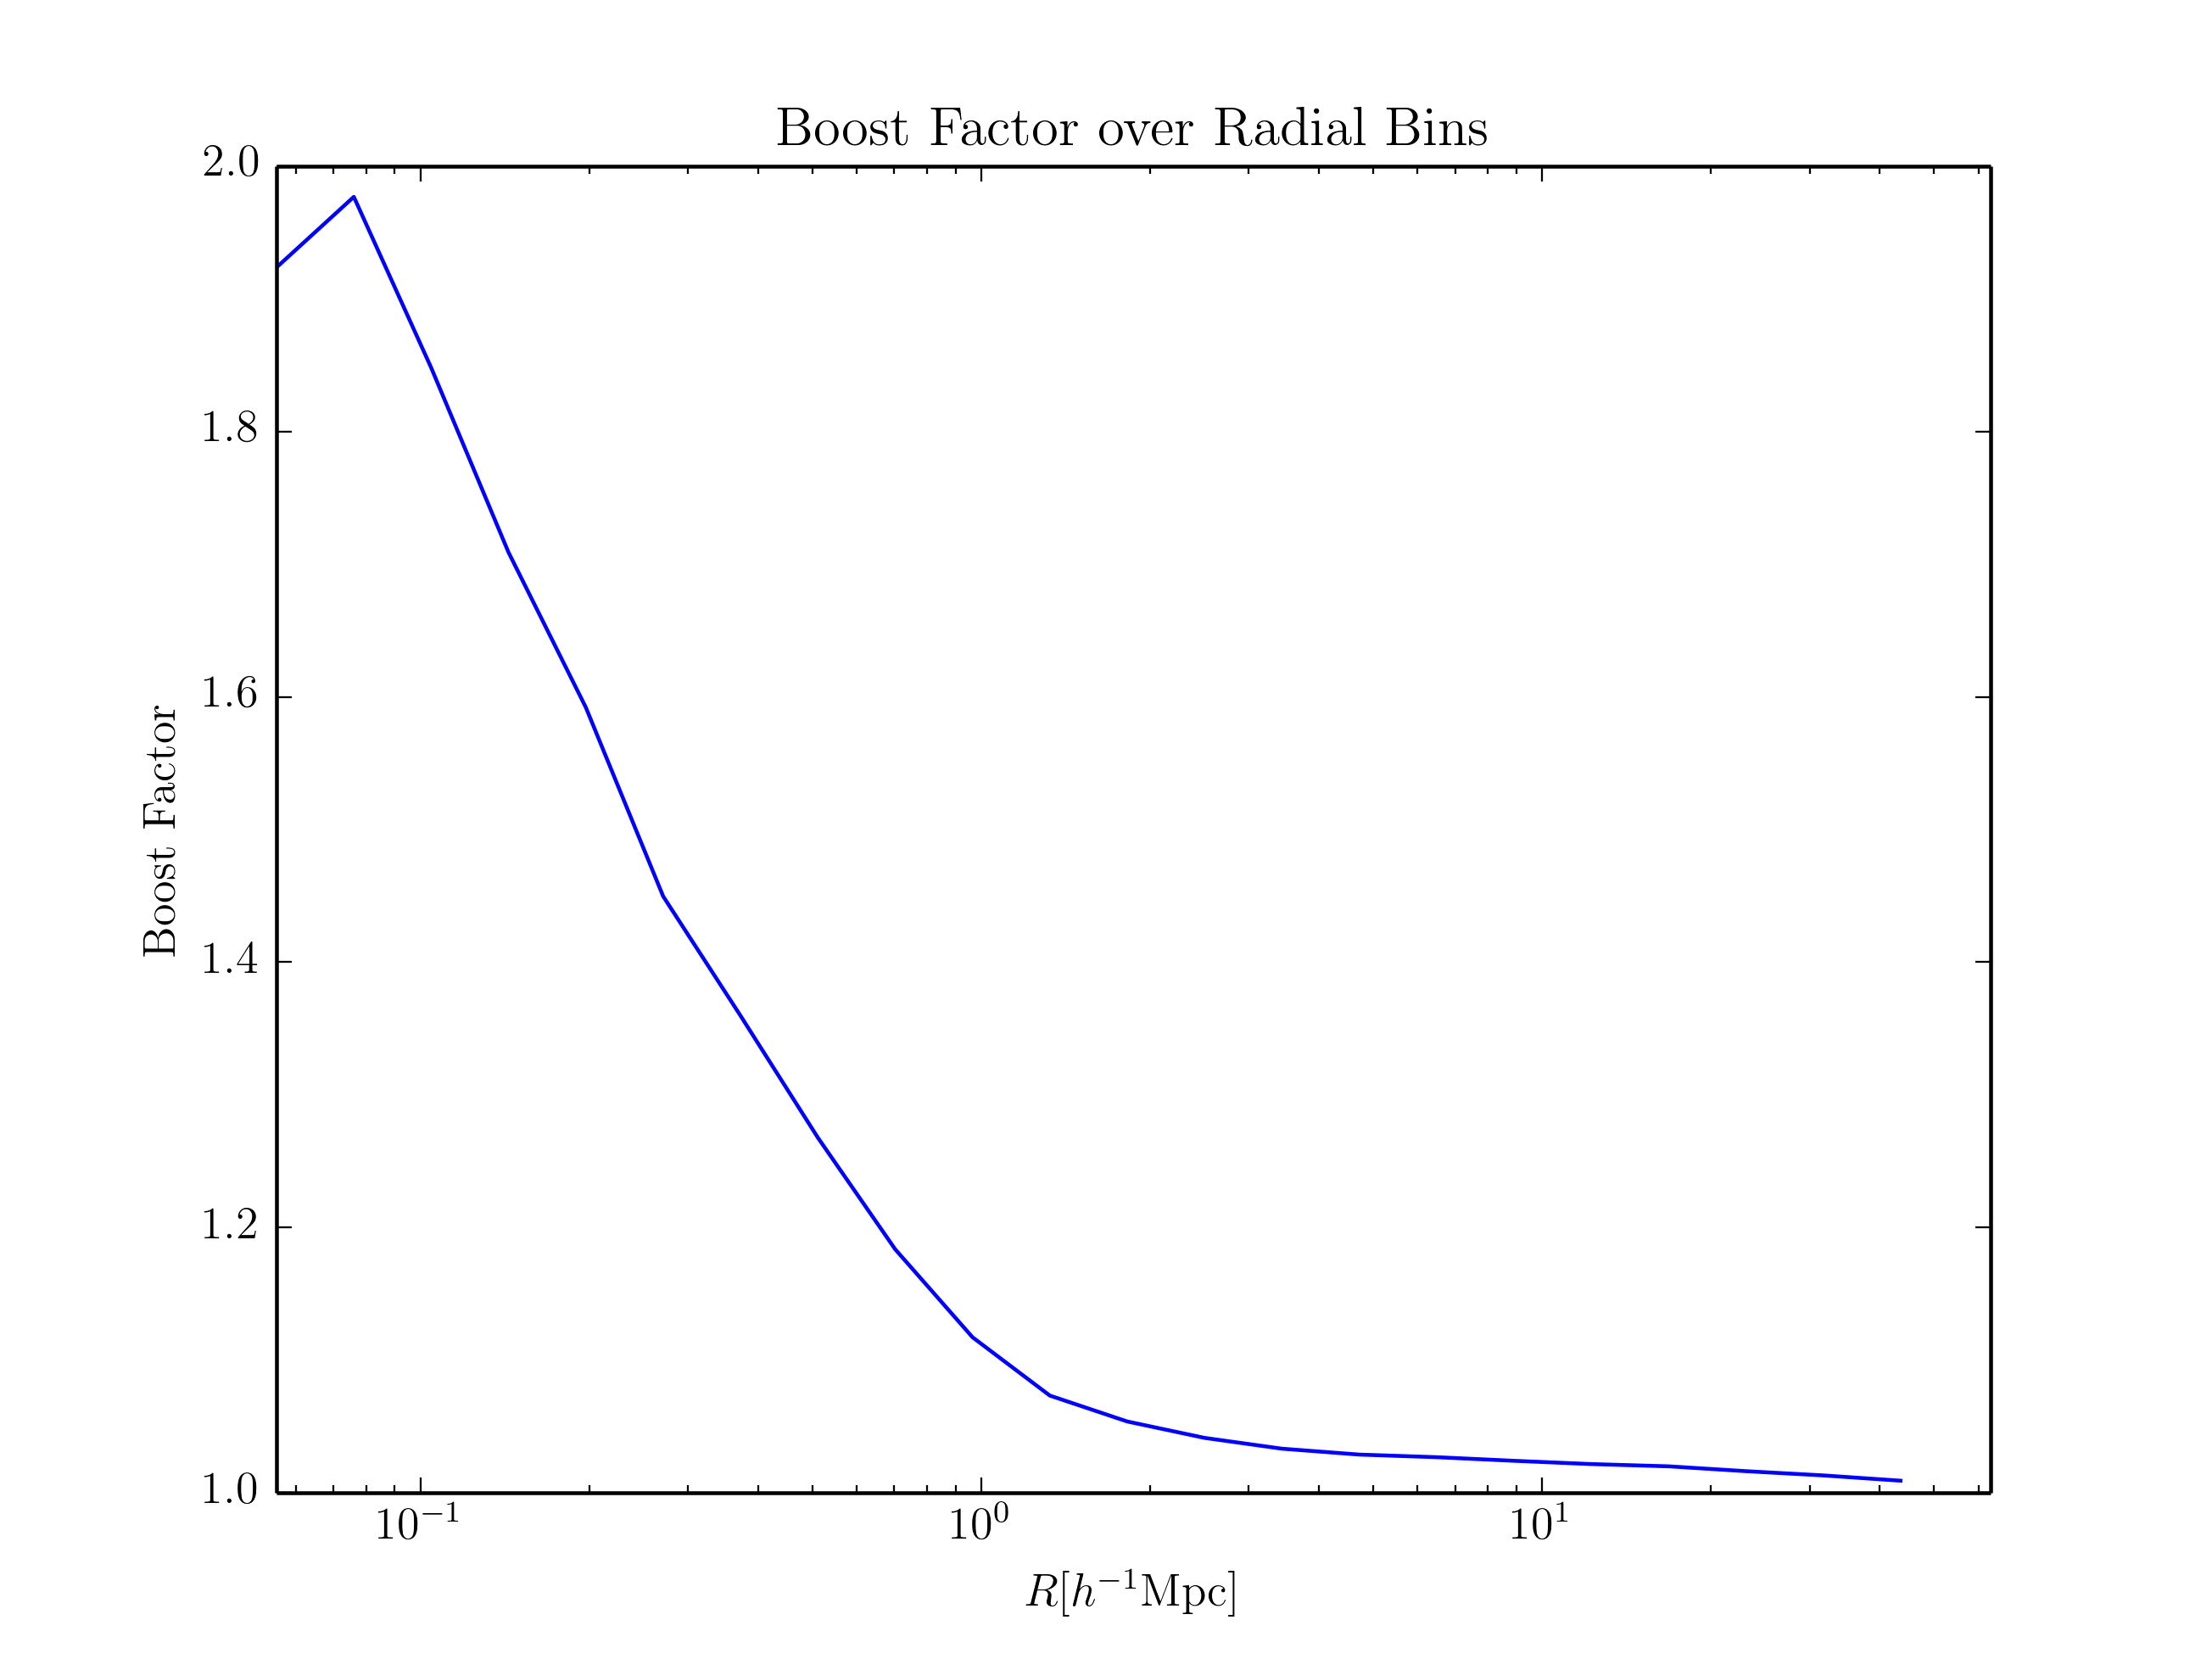
\includegraphics[width = \linewidth]{Boost_Factor}
		\label{fig:BoostFactor}
		\caption{Plot of the correction due to contamination of physically-associated galaxies (boost factor) over the radial bins. At small scales B(R)$>$1 and at large scales B(R)$\approx$1. Ideally the boost factor should remain close to 1. }
	\end{figure}
	
Figure 3 shows the boost factor for the parent sample. At small scales there is a large amount of contamination, and at large scales the correction approaches 1 as expected. In order to correct the weak lensing signal, we simply multiply the correction to the uncorrected signal.


\subsubsection{Photo-z Scatter}
Without photo-z errors, the observed tangental shear $\gamma_t$ can be related to $\Delta \Sigma$ by eq (\ref{eq:DeltaSigma}).  The redshift calibration bias comes from the misestimation of $\Delta\Sigma(R)$ due to photo-z scatter.
Using a subset of the source galaxies that were measured with spec-z, the correction factor for this effect can essentially be calculated as:
	\begin{equation}\label{eq:PhotoZ}
		b_z (z_{lens}) + 1 \equiv \frac{\widetilde{\Delta\Sigma}} {\Delta\Sigma},
	\end{equation}
where $\widetilde{\Delta\Sigma}$ is the lensing signal estimated using photo-z, and $\Delta\Sigma$ is the weak lensing signal using spec-z.

This bias can be used to corrected for a single lens redshift. In order to correct a sample clusters, an estimate of the average bias for the lens clusters was calculated.  

Further discussion of the photo-z correction has been discussed in great detail in \cite{2012MNRAS.420.3240N}.	

\subsubsection{Imperfect PSF Correction}
Another correction we need to apply is for imperfect Point Spread Function (PSF) correction in galaxy shape measurement. The contamination due to an imperfect PSF correction can be estimated by using the lensing signal around random points.
For each other subsamples, the large and small ellipticity, we calculated random signals of tangential shear and 45-degree rotated shear. These values are subtracted from the original weak lensing signal. 

\subsubsection{Covariance Matrices}\label{fig:Cov}
	\begin{figure*}[ht]
		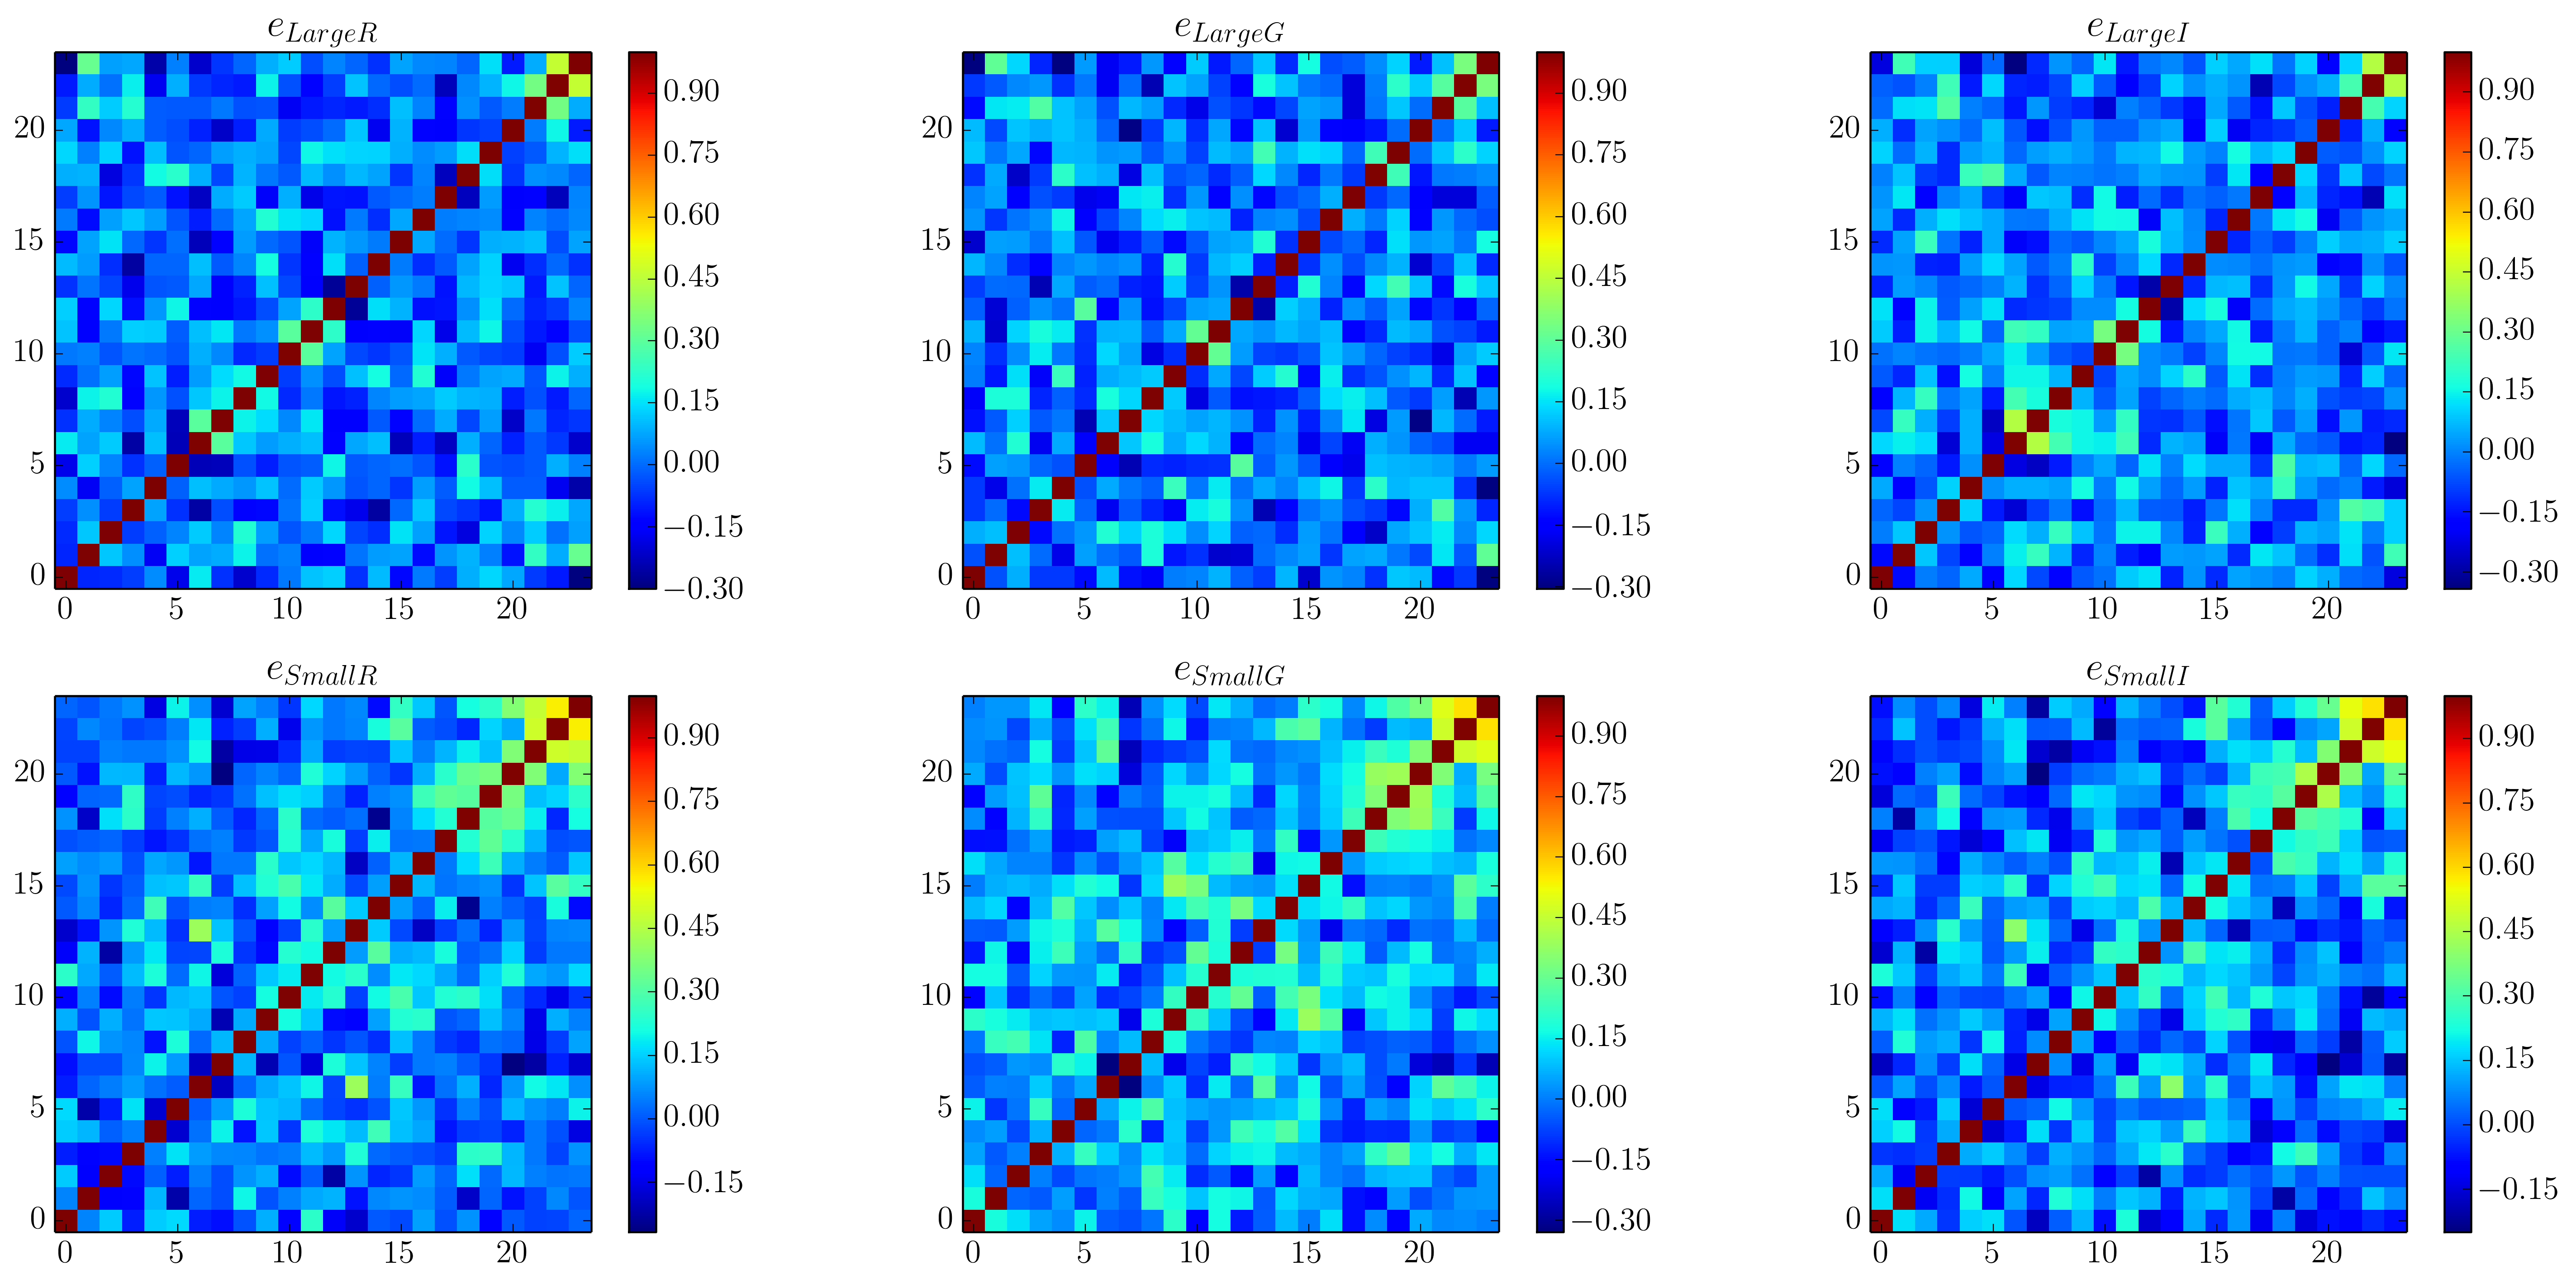
\includegraphics[width = \linewidth]{Correlation_Subsamples}
		\caption{This figure plots the various correlation matrices of the 6 subsamples, estimated by using 83 jackknife subsamples. The top row contains the large subsamples, and the bottom row displays the small subsamples. In general the correlation fluctuates around zero.}
	\end{figure*}
Each of the six subsamples were divided into 83 jackknife subsamples in order to calculate the error.This process of calculating the jackknife resampling includes removing one of the 83 subsamples, then calculating the average weak lensing signal of the remaining 82 subsamples and then calculating an average. This process is done 83 times and leaves us an array containing the average weak lansing signal of the 83 subsamples. This method allows a much more accurate value of the variation of the data points.The covariance matrix of jackknife covariance, which is defied as
	\begin{equation}
		\Delta\Sigma_{\mathrm{Variance}} = \frac{n-1} {n} A^TA
	\end{equation}
where $A$ is the matrix containing the 83 weak lensing signals minus the average of the weak lensing signal using the jackknife subsampling method, and $A^T$ is the transpose of that matrix.  The square-root of the diagonal of this matrix was used to determine the error bars of the weak lensing signals.

Once the covariance matrix is calculated, the correlation matrix can be calculated. The correlation can be calculated by:
	\begin{equation}
		\mathrm{Correlation} = \frac{\Delta\Sigma_{\mathrm{Variance} i, j}} {\sqrt{{\Delta\Sigma_{\mathrm{Variance} i, i}  {\Delta\Sigma_{\mathrm{Variance} j, j}} }}},
	\end{equation}
where the subscripts $i$ and $j$ represent the rows and columns of the terms in the covariance matrix. The plot of the correlation of is shown in Figure 4.


At small values of R the radial bins are not correlated, and at larger values of R the correlation is non-zero.
	
\subsection{Clustering Signal} 
Halo bias can be observed as the amplitude of clustering signal. If the clustering amplitude between subsamples is significantly different, it is the evidence of assembly bias. The clustering signal can be defined as:
	\begin{equation}
		w_p (\mathrm{R}) = \frac{DD(\mathrm{R})} {RR(\mathrm{R})} - 1,
	\end{equation}
DD represents the number of cluster pairs with the separation R, and RR is the number of pairs of random points with the separation R. The fractional difference between these cluster pairs and random pairs is what we observe as the clustering signal which tells us how likely a cluster is to form at some separation from another cluster. Naturally the clustering signal is expected to have a negative slope.

\section{Results}
	\begin{figure*}[h]
			\includegraphics[width = \linewidth]{StageSixSubSamplePlot_BMEM}
		\caption{This figure displays the three corrections being applied to the uncorrected weak lensing signals, tangental and 45-degree rotated shear. The corrections in general have boosted the signal of the E-Mode and shrunk the error bars.}
		\label{fig:StageCorrections}
	\end{figure*}

Figure \ref{fig:StageCorrections} shows the tangental (E-Mode) and the 45-degree rotated shear (B-Mode) and their respective corrections. The E-Mode was corrected with a boost correction, photo-z correction, and a random signal correction. The B-Mode was corrected with a random signal. The E-Mode shows how the dark matter distributes. At small scales the plot shows how dark matter distributes within a cluster, and at large scales it shows how the dark matter is distributed throughout neighboring clusters. The plot of B-Mode is theoretically predicted to be 0. The plot of B-Mode on the second and last rows of Figure 5 fluctuates around 0 as expected. The $\chi^2$, the sum of the ratio of the squares between the B-Mode and the B-Mode Error, of B-Mode is also less than one.
	\begin{figure*}[h]
		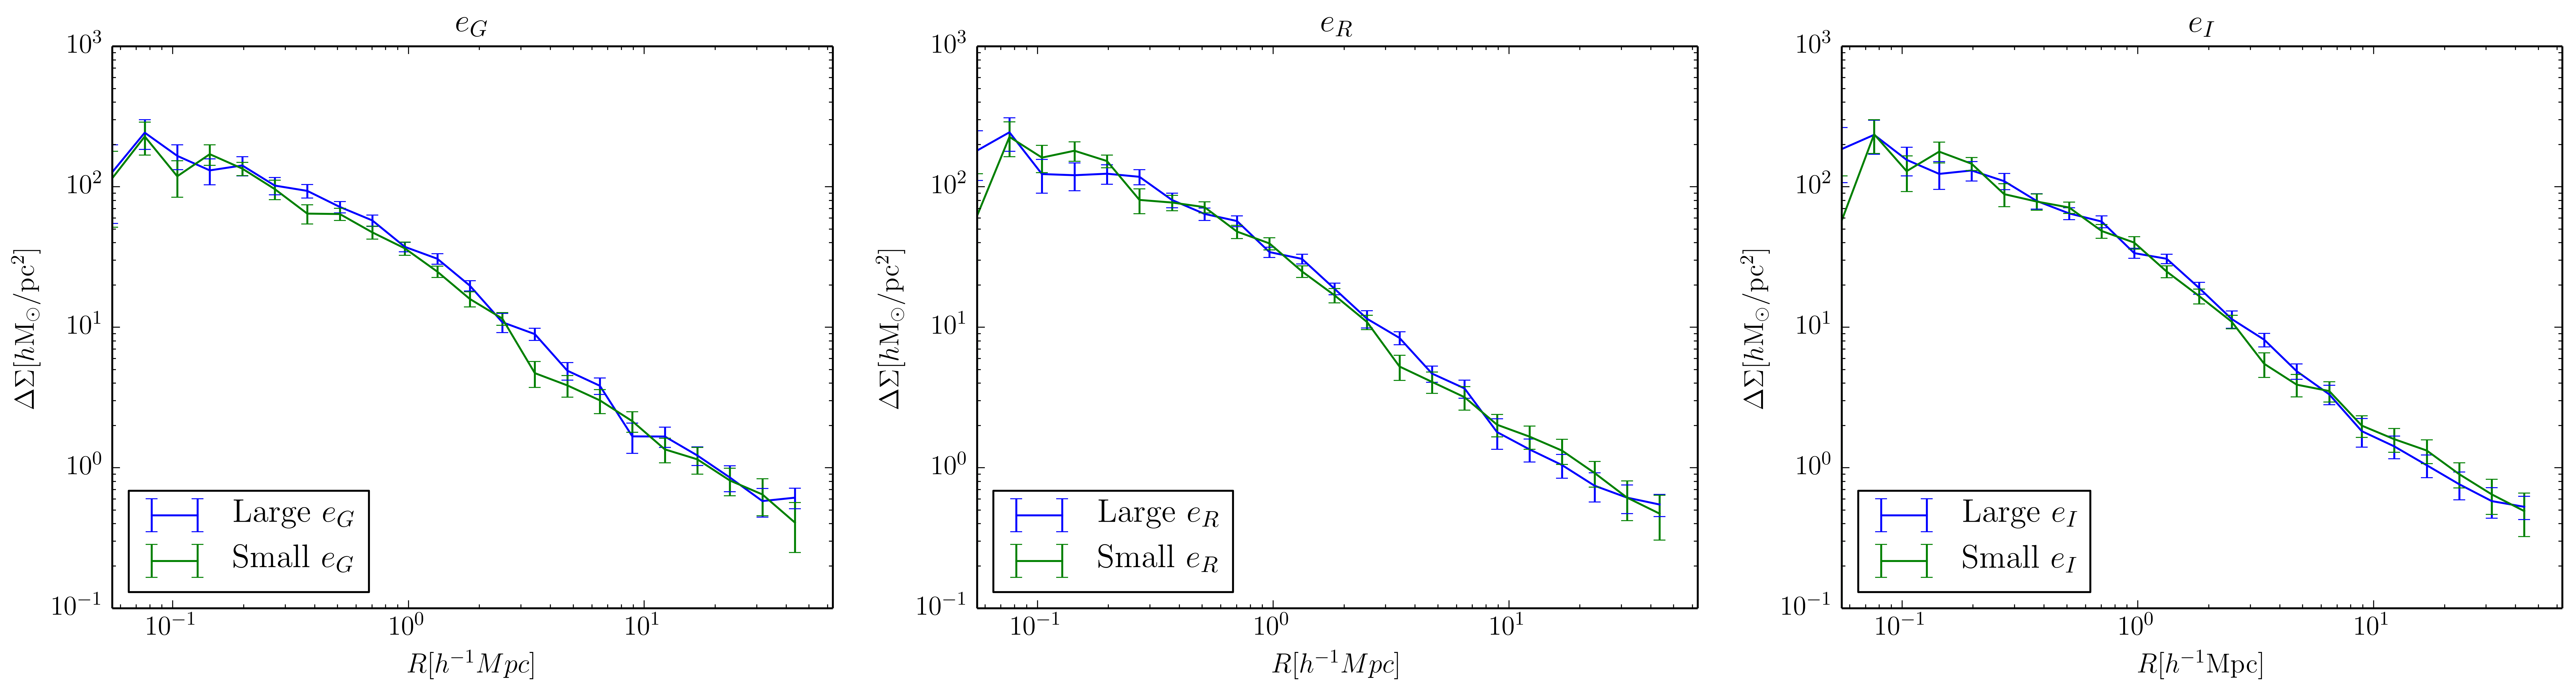
\includegraphics[width = \linewidth]{SixSubSamplePlotCorrectedEM}
		\caption{Plots of the corrected weak lensing signals of the 6 subsamples. The first panel contains the large and small ellipticity of the g-band, the second panel contains the large and small ellipticity of the r-band, and the last panel contains the large and small ellipticity of the i-band.}
		\label{fig:CorrectedSubsamplesWL}
	\end{figure*}

From the plots on Figure \ref{fig:CorrectedSubsamplesWL} it can be seen that the subsamples have the same mass. This is because at scales below 10 $h^{-1} \mathrm{Mpc}$ the two plots do not significantly deviate from each other. $\Delta\Sigma$ in indicative of the dark matter distribution of the clusters, if two subsamples have the similar $\Delta\Sigma$'s then those clusters have the same mass as most of the ass of galaxy clusters is dark matter. At large scales, above 10 $h^{-1} \mathrm{Mpc}$, the two subsamples do not deviate away from each other and are well within their error bars. The consequence of this is that BCG ellipticity does not induce assembly bias.

	\begin{figure*}[h] \label{fig:Cluster}
	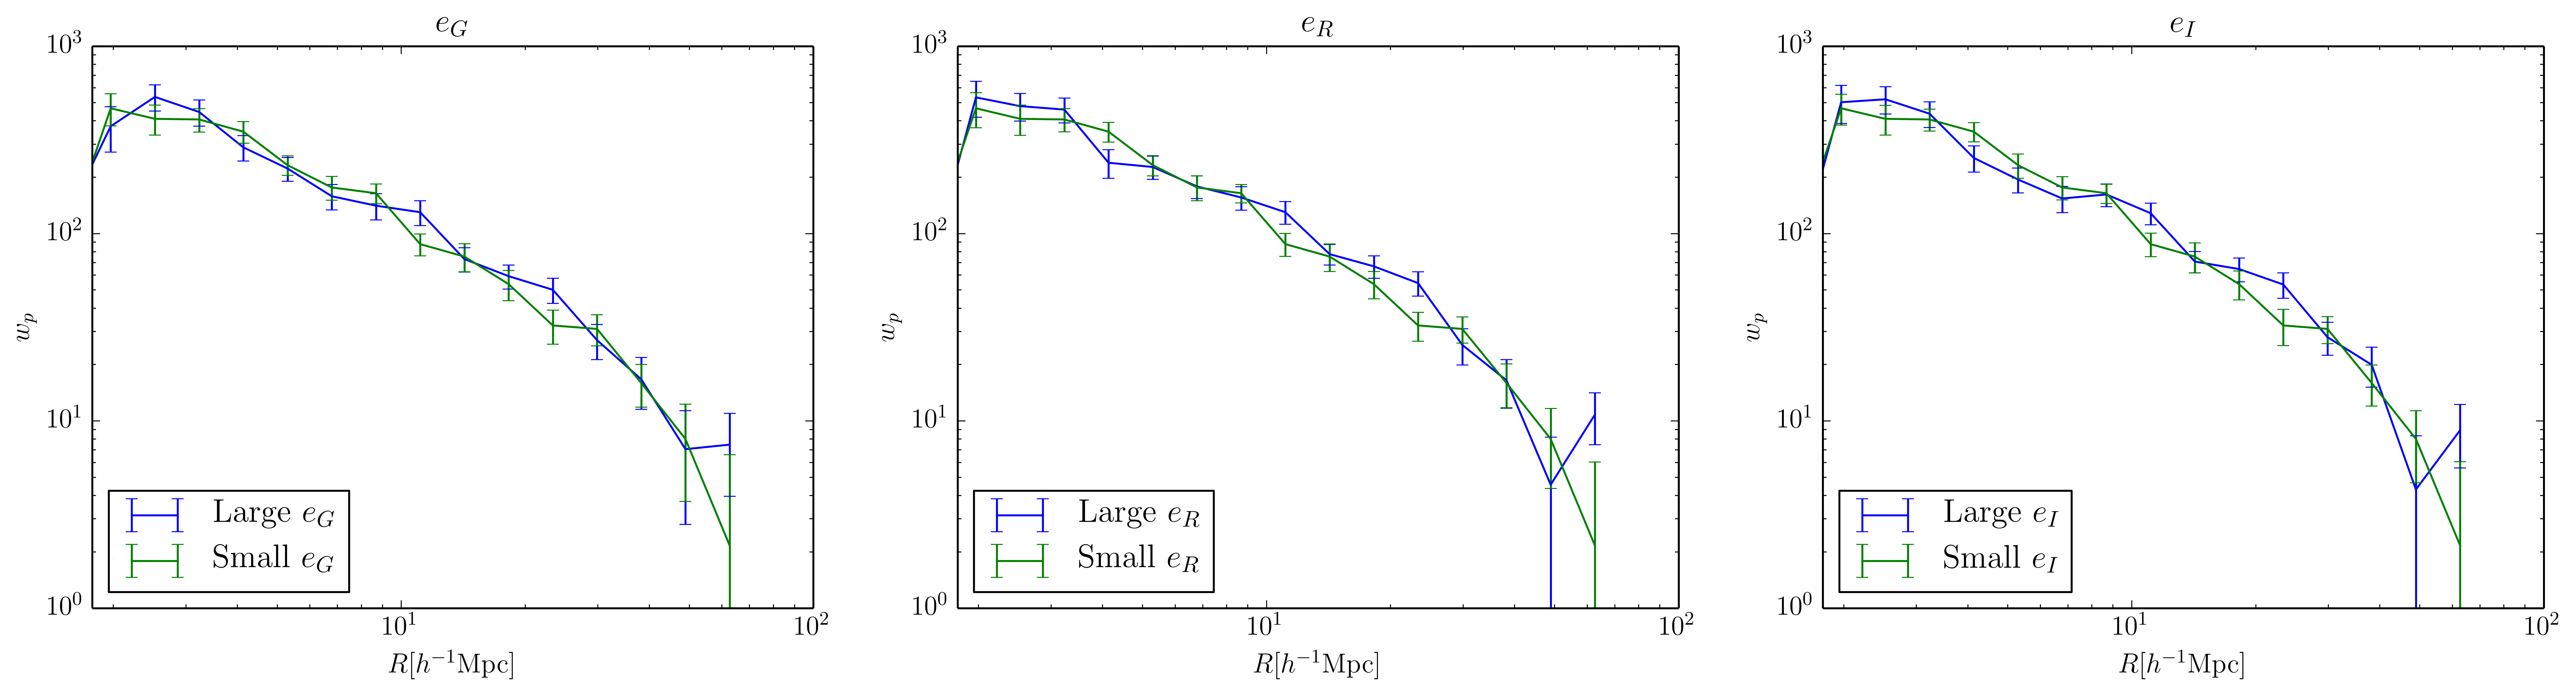
\includegraphics[width = \linewidth]{SixSubSamplePlot_From_Zodiac_Combined}
		\caption{The clustering signal which plots the probability of how clusters will form given a separation distance (R). From both large and small scales it can be seen that the two subsamples behave similarly. This means that there is no evidence of assembly bias within these clusters}
	\end{figure*}
Figure 7 plots he clustering signal. At both large and small scales it behaves similarly to the weak lensing signal in the sense that both subsamples do not display any significant deviation at large and small scales. Because of this we can say we did not detect any assembly bias in this sample of clusters.

\section{Discussion}
It is predicted that dark matter halo ellipticity correlates with bias. (\cite{2012JCAP...05..030S}) If BCG ellipticity correlates with the dark matter halo ellipticity, assembly bias should be detected. However, our subsamples did not show that BCG ellipticity induces assembly bias which might indicate hat BCG ellipticity and dark matter halo ellipticity are not correlated. In the future, other galaxy cluster properties that are predicted cause assembly bias could be studied such as BCG color, and dark matter concentration. In the future, data from the Hyper Suprime-Cam (HSC) or the upcoming Wide Field Infrared Survey Telescope (WFIRST) could be used to reinvestigate this project with their much deeper surveys.

\section{Conclusion}
In this project, 8,648 galaxy clusters from the SDSS redMaPPer catalog were used to detect assembly bias. Theory has shown that assembly bias can depend on the ellipticity of dark matter halos. Thus we created subsamples based on BCG ellipticity based on the assumption that there exists a correlation between BCG ellipticity and halo ellipticity. The weak lensing signal of these galaxy clusters were calculated in order to verify mass equivalence and assembly bias. At small scales, $<$ 10 $h^{-1} \mathrm{Mpc}$ the plots of the weak lensing signal should be the same. If the two plots have the same behavior, then their masses are equivalent. At large scales, $>$10 $h^{-1} \mathrm{Mpc}$ a change in the weak lensing signal of the subsamples will indicate whether or not assembly bias is present, because at this scale we are probing the dark matter of neighboring clusters. It was found that BCG ellipticity does not induce assembly bias because there was no significant differences in the weak lensing and clustering signals at large scales. In conclusion, BCG ellipticity does not affect the dark matter distribution.

\bibliographystyle{apj}
\bibliography{Final_Draft_APJ}
%\appendix

%\section{Appendix material}

\end{document}

